\documentclass{article}

% Language setting
\usepackage[english]{babel}

% Set page size and margins
\usepackage[a4paper,top=2cm,bottom=2cm,left=3cm,right=3cm,
	marginparwidth=1.75cm]{geometry}

% Useful packages
\usepackage{amsmath}
\usepackage{graphicx}
\usepackage[colorlinks=true, allcolors=blue]{hyperref}

% For inline enumerations
\usepackage{enumitem}

\usepackage{tikz}
\usetikzlibrary{shapes,arrows,positioning,fit,backgrounds}

\title{
	Evaluating the Vertical and Horizontal Read and Write Scalability of 
	MobilityDB
	\\[1ex] \large Bachelor's Thesis Exposé}
\author{Eryk Karol Kściuczyk}
\date{} % This removes the date

\begin{document}
\maketitle


% Context
Spatio-temporal databases are increasing in popularity due to increased
production of such data by numerous IoT devices.
As the need for such databases increases, developers try to reach for 
open-source and familiar solutions.
MobilityDB, built on top of the spatial extension PostGIS, extends PostgreSQL's 
capabilities regarding spatio-temporal aspects.
Previous research has shown that the MobilityDB extension can be partially used
in conjunction with Citus, a PosgreSQL extension, which provides horizontal
scalability options.\footnote{
Bakli, Sakr and Zimanyi, "MobilityDB: A Mobility Database Based on PostgreSQL 
and PostGIS," ACM Transactions on Database Systems (TODS), Volume 45, Issue 4, 
Article No. 19, Pages 1-42, December 6, 2020
}
It does it by sharding data across multiple nodes while retaining the rich
features of PostgreSQL. While specific queries and their runtimes have been 
evaluated\footnote{
Bakli, Sakr, and Zimanyi, "Distributed Mobility Data Management in MobilityDB," 
Proceedings of the 2020 21st IEEE International Conference on Mobile Data
Management (MDM), June 2020
},
the vertical and horizontal scalability of the platform has not been fully
explored and measured.

% Problem Statement
MobilityDB's distributed capabilities, enabled by integration with Citus, claim
to enhance scalability.
% TODO: try to shorten this section into one or two sentences
% mention the unexplored angles
However, the platform's ability to efficiently scale read and write operations
under real-world workloads has not been rigorously evaluated as current research
has primarily focused on optimizing and measuring read query performance.
However, write throughput—critical for handling high-ingest workloads typical 
of IoT applications—remains underexplored, especially in scenarios involving
concurrent writes across distributed nodes.
Questions remain about latency, throughput, and scalability in vertical and
horizontal configurations when handling realistic spatio-temporal datasets.

% Solution Approach
In this thesis we aim to benchmark the vertical and horizontal scalability
regarding both read and write operations with generated spatio-temporal data to
measure metrics like request latency and write throughput.
% TODO: shorten by merging it with the next sections that also mention it
We plan to deploy MobilityDB on single-node and multi-node setups.
Additionally, we will analyze how query options affect impact on the performance
in different configurations.
Afterwards, we want to compare scalability trade-offs between vertical and
horizontal approaches.

% Aspired Implementation
Benchmarking data will be generated using a custom data generation tool
specifically developed for this study.
The tool will simulate the movement and locations of birds, chosen due to their
seasonal migration patterns, localized movements within standard habitats,
varying flight heights and times.
%
We will compare the performance of MobilityDB combined with Citus on different
hardware configurations using Google Compute Engine service on Google Cloud
Platform.
We will evaluate several scenarios, including vertically scaling a single node
and scaling out by distributing MobilityDB across several instances.

\begin{figure}[ht]
    \centering
    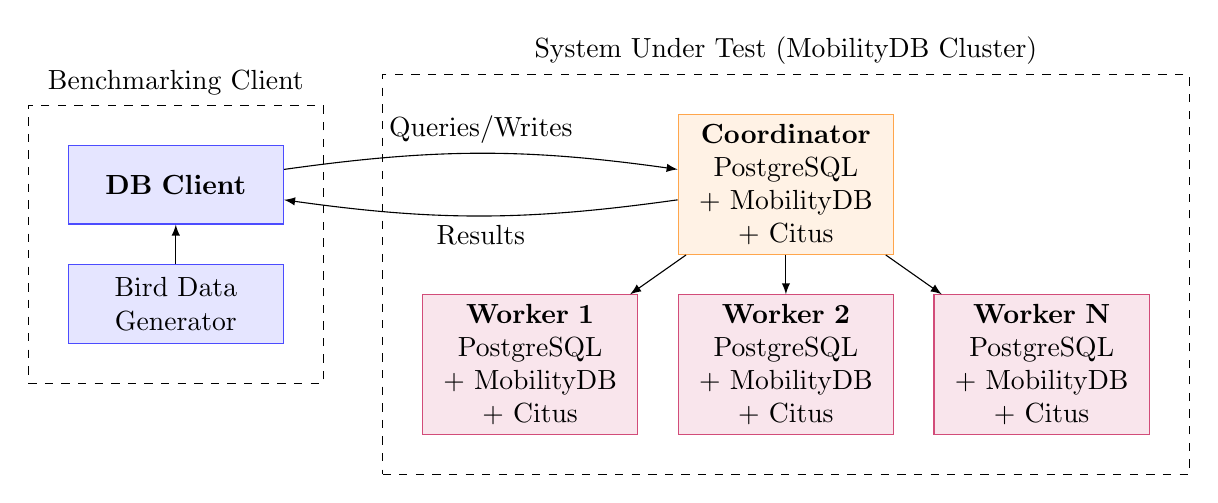
\begin{tikzpicture}[
        node distance=0.5cm,
        box/.style={
            rectangle,
            draw,
            text width=2.5cm,
            minimum height=1cm,
            align=center
        },
        client/.style={
            box,
            fill=blue!10,
            draw=blue!70
        },
        coordinator/.style={
            box,
            fill=orange!10,
            draw=orange!70,
        },
        worker/.style={
            box,
            fill=purple!10,
            draw=purple!70
        },
        group/.style={
            rectangle,
            draw,
            dashed,
            inner sep=0.5cm
        },
        arrow/.style={
            ->,
            >=latex
        }
    ]
    % Client components
    \node[client] (db_client) {\textbf{DB Client}};
    \node[client, below=of db_client] (datagen) {Bird Data Generator};
    % Client connections
    \draw[arrow] (datagen) -- (db_client);
    % Coordinator node
    \node[coordinator, right=5cm of db_client] (cn) {
         \textbf{Coordinator}\\PostgreSQL + MobilityDB + Citus};
    % Worker nodes
    \node[worker, below=of cn] (w2) {
	    \textbf{Worker 2}\\PostgreSQL + MobilityDB + Citus};
    \node[worker, left=of w2] (w1) {
	    \textbf{Worker 1}\\PostgreSQL + MobilityDB + Citus};
    \node[worker, right=of w2] (w3) {
	    \textbf{Worker N}\\PostgreSQL + MobilityDB + Citus};
    % Connections to workers
    \draw[arrow] (cn) -- (w1);
    \draw[arrow] (cn) -- (w2);
    \draw[arrow] (cn) -- (w3);
    % Client to SUT connections
    \draw[arrow] (db_client) to[bend left=8] node[above] {Queries/Writes} (cn);
    \draw[arrow] (cn) to[bend left=8] node[below] {Results} (db_client);
    
    % Group boxes
    \begin{pgfonlayer}{background}
        \node[group, fit=(db_client) (datagen)] (client) {};
        \node[above] at (client.north) {Benchmarking Client};

        \node[group, fit=(cn) (w1) (w2) (w3)] (sut) {};
        \node[above] at (sut.north) {System Under Test (MobilityDB Cluster)};
    \end{pgfonlayer}
    \end{tikzpicture}
    \caption{
	Benchmarking client will use generated bird movement data and execute
	the workload against System Under Test (MobilityDB cluster).
	The cluster consists of a coordinator and multiple worker, each running
	PostgreSQL with MobilityDB and Citus extensions. 
    }
    \label{fig:image}
\end{figure}

% Analysis/ Evaluation
% TODO:
% - Make it shorter
% - Shrink the diagram
For evaluation of our results, we will employ multiple statistical and
visualization approaches to ensure comprehensive analysis of the system's
performance characteristics. 
%
Query latencies and throughput measurements will be analyzed using confidence
intervals (95\% CI) to account for performance variability in distributed
systems. 
%
To visualize the distribution of latencies across different scaling
configurations, we will utilize Empirical Cumulative Distribution Function
(ECDF) plots, to reveal performance patterns and tail latencies.
%
For write throughput analysis, we will present time series plots showing
sustained throughput over extended periods, accompanied by statistical summaries
including median, 95th, and 99th percentiles.
%
In order to validate the statistical significance of performance differences
between vertical and horizontal scaling approaches, we will conduct paired
t-tests where appropriate.
%
Each benchmark configuration will be run multiple times with sufficient duration
(minimum 30 minutes per run) to ensure statistical reliability and to capture
any performance degradation or variance over time.
\end{document}
